\newcommand{\NWtarget}[2]{\hypertarget{#1}{#2}}
\newcommand{\NWlink}[2]{\hyperlink{#1}{#2}}
\newcommand{\NWtxtMacroDefBy}{Fragment defined by}
\newcommand{\NWtxtMacroRefIn}{Fragment referenced in}
\newcommand{\NWtxtMacroNoRef}{Fragment never referenced}
\newcommand{\NWtxtDefBy}{Defined by}
\newcommand{\NWtxtRefIn}{Referenced in}
\newcommand{\NWtxtNoRef}{Not referenced}
\newcommand{\NWtxtFileDefBy}{File defined by}
\newcommand{\NWtxtIdentsUsed}{Uses:}
\newcommand{\NWtxtIdentsNotUsed}{Never used}
\newcommand{\NWtxtIdentsDefed}{Defines:}
\newcommand{\NWsep}{${\diamond}$}
\newcommand{\NWnotglobal}{(not defined globally)}
\newcommand{\NWuseHyperlinks}{}
\documentclass[12.0pt]{report}
%\usepackage[a4paper, left=2cm, right=2cm, top=2cm]{geometry}
\usepackage[text={19.0cm,24.5cm}]{geometry}
\usepackage{marginnote}

% https://stackoverflow.com/a/27243065/505306
% Making caption font smaller on figures and tables.
\usepackage{caption}
\captionsetup{font=footnotesize}

% Forcing line-breaks in url's
% https://tex.stackexchange.com/questions/3033/forcing-linebreaks-in-url
\usepackage[hyphens]{url}



\usepackage{asymptote}
\usepackage{asypictureB}
\renewcommand\asydir{asytmp} 

%-------------------------------------------------------------------------------
%\usepackage[left,pagewise]{lineno}
%\linenumbers
\usepackage[framemethod=TikZ]{mdframed}
\usepackage{wrapfig}
\usepackage{amsthm}
\usepackage{bm}
\usepackage{amsfonts}
\usepackage{minted}
% ------------------------------------------------------------------------------
\usepackage[toc,page]{appendix}

%-------------------------------------------------------------------------------
%https://tex.stackexchange.com/a/278199/17858
% For aligning itemize environments to left
\usepackage{enumitem}
\mdfsetup{%
   middlelinecolor=red,
   middlelinewidth=0pt,
   roundcorner=10pt}

\mdfdefinestyle{MyFrame}{%
    linecolor=black,
    outerlinewidth=0.1pt,
    roundcorner=0pt,
    innertopmargin=14pt,
    innerbottommargin=4pt,
    innerrightmargin=4pt,
    innerleftmargin=4pt,
        leftmargin = 4pt,
        rightmargin = 4pt,
    %backgroundcolor=gray!50!white}
     }
     
%-------------------------------------------------------------------------------

%\usepackage{fourier}  % Another nice font for the main text

% Useful for breaking long lines of text https://tex.stackexchange.com/a/176780
% in a table

\usepackage{array}
\usepackage{makecell}

\renewcommand\theadalign{bc}
\renewcommand\theadfont{\bfseries}
\renewcommand\theadgape{\Gape[4pt]}
\renewcommand\cellgape{\Gape[4pt]}
\usepackage{makecell}


\definecolor{theocol}{RGB}{255, 222, 228}
\newtheorem{theo}{Theorem}
\newenvironment{ftheo}
  {\begin{mdframed}[style=MyFrame,nobreak=true, backgroundcolor=theocol]\begin{theo}}
  {\end{theo}\end{mdframed}}


\definecolor{lemcol}{RGB}{226, 255, 220}
\newtheorem{lem}{Lemma}
\newenvironment{flem}
  {\begin{mdframed}[style=MyFrame,nobreak=true, backgroundcolor=lemcol]\begin{lem}}
  {\end{lem}\end{mdframed}}

\definecolor{corcol}{RGB}{227, 227, 227}
\newtheorem{cor}{Corollary}
\newenvironment{fcor}
  {\begin{mdframed}[style=MyFrame,nobreak=true, backgroundcolor=corcol]\begin{cor}}
  {\end{cor}\end{mdframed}}

\definecolor{propcol}{RGB}{227, 227, 227}
\newtheorem{prop}{Proposition}
\newenvironment{fprop}
  {\begin{mdframed}[style=MyFrame,nobreak=true, backgroundcolor=propcol]\begin{prop}}
  {\end{prop}\end{mdframed}}

\definecolor{conjcol}{RGB}{248, 218, 194}
\newtheorem{conj}{Conjecture}
\newenvironment{fconj}
  {\begin{mdframed}[style=MyFrame,nobreak=true, backgroundcolor=conjcol]\begin{conj}}
  {\end{conj}\end{mdframed}}


\definecolor{notecol}{RGB}{255, 152, 149  }
\newenvironment{note}
  {\begin{mdframed}[style=MyFrame,nobreak=true, backgroundcolor=notecol]}
  {\end{mdframed}}

\usepackage{enumitem}

%-------------------------------------------------------------------------------
% https://tex.stackexchange.com/q/2291/17858
% if you want to create a new list from scratch
\newlist{alphalist}{enumerate}{1}
% in that case, at least label must be specified using \setlist
\setlist[alphalist,1]{label=\textbf{\Alph*.}}

%--------------------------------------------------------------------------------
\usepackage[english]{babel}
%\setlength{\voffset}{-0.75in}
\setlength{\headsep}{5pt}

%-------------------------------------------------------------------------------
\usepackage{blindtext}
\usepackage{lipsum}
\usepackage{textcomp}

%-------------------------------------------------------------------------------
\usepackage{filecontents}
\usepackage{parskip} 
\usepackage{tocloft}
\usepackage{graphicx}                             % Include images into pdf document 
\usepackage{tikz}                                 % Useful for the circled command. Don't remove!
\usepackage{multicol}                             % For lists in two or more columns

\usepackage[nokwfunc, ruled]{algorithm2e}
\newcommand\mycommfont[1]{\footnotesize\ttfamily\textcolor{blue}{#1}}
\SetCommentSty{mycommfont}
\SetKwComment{Comment}{$\triangleright$\ }{}
\usepackage[T1]{fontenc}
%-------------------------------------------------------------------------------
\usepackage{needspace}                % So that sections/code-blocks don't straddle two pages 
\usepackage{mathtools}
\usepackage{subfig}
\usepackage{etoolbox}
\usepackage{color}
\usepackage{pifont}
\setlength{\parindent}{20pt}
% For italicizing quotes: https://tex.stackexchange.com/a/288556/17858

%-------------------------------------------------------------------------------
\usepackage[utf8]{inputenc}
\usepackage{csquotes}
\renewcommand{\mkbegdispquote}[2]{\itshape}

%-------------------------------------------------------------------------------
% Convenience commands
\newcommand*\circled[1]{\tikz[baseline=(char.base)]{\node[shape=circle,draw,inner sep=2pt] (char) {#1};}}
\providecommand{\myceil}[1]{\left \lceil #1 \right \rceil }	% Ceil function
\providecommand{\myfloor}[1]{\left \lfloor #1 \right \rfloor }	% Floor function\renewcommand{\labelitemi}{\tiny$\blacksquare$}	
\newcommand\given[1][]{\:#1\vert\:}                             % for drawing the conditional probability `|` sign neatly.
\newcommand\RR{\mathbb{R}}					% Set of reals numbers
\newcommand\CC{\mathbb{C}}					% Set of complex numbers
\newcommand\ZZ{\mathbb{Z}}					% Set of integers
\newcommand\NN{\mathbb{N}}					% Set of naturals
\newcommand\rarr{\rightarrow}					% Rightarrow
\newcommand\larr{\leftarrow}					% Leftarrow
\newcommand\defeq{\coloneqq}					% := symbol
\renewcommand\tilde{ \: \thicksim \: }				% Sane tildas
\newmdenv[topline=false, bottomline=false, skipabove=\topsep,skipbelow=\topsep]{siderules}
%\setlength{\droptitle}{-18em}					% Eliminate the default vertical space
%\hypersetup{colorlinks=true,linkcolor=blue}


%-------------------------------------------------------------------------------
% Writing the text of a section immediately after section title
% Vedic and old british style where text immediately follows the 
% subsection number. https://tex.stackexchange.com/a/99177/17858
%\usepackage{titlesec}
%\titlespacing{\section}{0pt}{*0}{*0}
%\titlespacing{\subsection}{0pt}{*0}{*0}
%\titlespacing{\subsubsection}{0pt}{*0}{*0}
\usepackage[compact]{titlesec}
\titlespacing{\section}{0pt}{2ex}{1ex}
\titlespacing{\subsection}{0pt}{1ex}{0ex}
\titlespacing{\subsubsection}{0pt}{0.5ex}{0ex}
%\setlength{\parskip}{0.1cm} % Paragraph separation
\setlength{\parindent}{2em}

\titleformat*{\section}{\Huge\bfseries}
\titleformat{\subsection}[runin]{\normalfont\Large\bfseries}{\thesubsection}{0.5em}{}
\titleformat*{\subsubsection}{\Large\bfseries}
%{\normalfont\huge\bfseries}{\sectiontitlename\ \thesection:}{1em}{} 
%% Custom Literate Proof Commands:
%\newcommand{\newchunk}[2]{\section{#2}\label{sec:#1}\quad}
\newcommand{\newchunk}{\subsection{}\quad}
\newcommand{\refchunk}[1]{\ref{sec:#1}}
%\newcommand{\sect}[1]{\section{#1}\quad} 
%-------------------------------------------------------------------------------
% For centeriing the titile
% https://tex.stackexchange.com/a/290449/17858
\usepackage{titling}
\renewcommand\maketitlehooka{\null\mbox{}\vfill}
\renewcommand\maketitlehookd{\vfill\null}

%-------------------------------------------------------------------------------
% To express an idea in a crunchy way.
\newcommand{\crunchy}[1]{\lbrack{} \large \textit{#1} \normalsize \rbrack} 
%-------------------------------------------------------------------------------
\makeatletter
\def\@makechapterhead#1{%
  %%%%\vspace*{50\p@}% %%% removed!
  {\parindent \z@ \raggedright \normalfont
    \ifnum \c@secnumdepth >\m@ne
        \huge \bfseries \@chapapp\space \thechapter
        \par\nobreak
        \vskip 20\p@
    \fi
    \interlinepenalty\@M
    \Huge \bfseries #1\par\nobreak
    \vskip 40\p@
  }}
\def\@makeschapterhead#1{%
  %%%%%\vspace*{50\p@}% %%% removed!
  {\parindent \z@ \raggedright
    \normalfont
    \interlinepenalty\@M
    \Huge \bfseries  #1\par\nobreak
    \vskip 40\p@
  }}
\makeatother


\usepackage{fancyhdr}
\usepackage{datetime}

\fancyhf{}
\fancyfoot[L]{\today\ \currenttime}
\pagestyle{fancy}

% https://tex.stackexchange.com/a/458876/17858 rounded
% pink rectangles around an inline word
\newcommand{\sticker}[1]{\tikz[baseline=(X.base)]\node [draw=red,fill=pink!60,semithick,rectangle,inner sep=2pt, rounded corners=3pt] (X) { {\footnotesize \color{red} #1}};}


\newif\ifshowcode
\showcodetrue
\usepackage{latexsym}
\usepackage{listings}
\usepackage{color}
\definecolor{linkcolor}{rgb}{0, 0, 0.7}

\usepackage[%
backref,%
raiselinks,%
pdfhighlight=/O,%
pagebackref,%
hyperfigures,%
breaklinks,%
colorlinks,%
pdfpagemode=None,%
pdfstartview=FitBH,%
linkcolor={linkcolor},%
anchorcolor={linkcolor},%
citecolor={linkcolor},%
filecolor={linkcolor},%
menucolor={linkcolor},%
pagecolor={linkcolor},%
urlcolor={linkcolor}%
]{hyperref}


% % %-------------------------------------------------------------------------------
% % %https://tex.stackexchange.com/a/141662/17858
% % %reset numbering of theorems, lemmas and corollaries every chapter 
% \usepackage{chngcntr}
% \counterwithin*{theo}{chapter} 
% \counterwithin*{lem}{chapter} 
% \counterwithin*{cor}{chapter} 


%% For making lualatex work with asymptote
%% ripped from https://tex.stackexchange.com/a/376412/17858
\usepackage{ifluatex}
\ifluatex
\makeatletter
\def\asy@input@graphic{%
  \ifASYinline
    \IfFileExists{"\AsyFile.tex"}{%
      \catcode`:=12\relax
      \@@input"\AsyFile.tex"\relax
    }{%
      \PackageWarning{asymptote}{file `\AsyFile.tex' not found}%
    }%
  \else
    \IfFileExists{"\AsyFile.\AsyExtension"}{%
      \ifASYattach
        \ifASYPDF
          \IfFileExists{"\AsyFile+0.pdf"}{%
            \setbox\ASYbox=\hbox{\includegraphics[hiresbb]{\AsyFile+0.pdf}}%
          }{%
            \setbox\ASYbox=\hbox{\includegraphics[hiresbb]{\AsyFile.pdf}}%
          }%
        \else
          \setbox\ASYbox=\hbox{\includegraphics[hiresbb]{\AsyFile.eps}}%
        \fi
        \textattachfile{\AsyFile.\AsyExtension}{\phantom{\copy\ASYbox}}%
        \vskip-\ht\ASYbox
        \indent
        \box\ASYbox
      \else
        \ifASYPDF
          \includegraphics[hiresbb]{\AsyFile.pdf}%
        \else
          \includegraphics[hiresbb]{\AsyFile.eps}%
        \fi
      \fi
    }{%
      \IfFileExists{"\AsyFile.tex"}{%
        \catcode`:=12
        \@@input"\AsyFile.tex"\relax
      }{%
        \PackageWarning{asymptote}{%
          file `\AsyFile.\AsyExtension' not found%
        }%
      }%
    }%
  \fi
}
\makeatother
\fi

%%%%%%%%%%%%%%%%%%%%%%%%%%%%%%%%%%%%%%%%%%%%%%%%%%%%%%%%%%%%%%%%
%% for setting program fonts
%% As recommended by http://nepsweb.co.uk/docs/progfonts.pdf
%% He recommends bera mono. 
%%\usepackage[scaled]{beramono}
%%\usepackage[T1]{fontenc}

%% I liked txtt also. 
%%\renewcommand{\ttdefault}{txtt}
\usepackage{listings}
\usepackage{inconsolata}
\usepackage[T1]{fontenc}
\lstset{basicstyle=\normalsize\ttfamily,breaklines=true}
\lstset{framextopmargin=50pt,frame=bottomline}
\lstset{language=Python}   



\usepackage{harpoon}% <---


%%% Super useful for marking todo notes, ripped from here: 
%%% https://tex.stackexchange.com/a/178806/17858
\usepackage{xargs}                      % Use more than one optional parameter in a new commands
\usepackage[colorinlistoftodos,prependcaption,textsize=tiny]{todonotes}
\newcommandx{\UNSURE}[2][1=]{\todo[linecolor=blue,backgroundcolor=blue!25,bordercolor=blue,#1]{#2}}
\newcommandx{\TODO}[2][1=]{\todo[linecolor=red,backgroundcolor=red!25,bordercolor=red,#1]{#2}}

\usepackage{kantlipsum}
\usepackage{fancyvrb}
\usepackage{setspace}
\newenvironment{CVerbatim}
 {\singlespacing\center\BVerbatim}
 {\endBVerbatim\endcenter}

\usepackage{tocloft}
\renewcommand{\cftpartfont}{\LARGE\itshape} % Part title in Huge Italic font
\usepackage{hyperref}
\usepackage{etoolbox}
% Better formatting of backticks in 
% verbatim environment. 
\usepackage{upquote}

% page numbering at top right
\usepackage{fancyhdr}
\pagestyle{fancy}
\fancyhf{}
\fancyhead[R]{\thepage}

\begin{document}
\begin{titlepage}
	\centering
        {\Huge Analyses of Experimental Heuristics for Package-Handoff Type Problems\\}
        \vspace{20mm}
        {\Large Gaurish Telang}
\end{titlepage}
\pagenumbering{arabic}
\setcounter{page}{2} 
\setcounter{tocdepth}{1}
\tableofcontents
\addtocontents{toc}{~\hfill\textbf{Page}\par}

\chapter{Overview}

How do you get a package from point $A$ to point $B$ with a fleet of carrier drones each 
capable of various maximum speeds? This is the question we try to answer in some of  
its various avatars by developing algorithms, heuristics, local optimality heuristics 
and lower-bounds. 

Specifically, we are given as input the positions $P_i$ of $n$ drones (labelled 1 through $n$) 
in the plane each capable of a maximum speed of $u_i$. Also given is a package present 
at $S$ that needs to get to $T$. Each drone is capable of picking up the package and 
flying with speed $u_i$ to another point to hand the package off to another drone. 

\begin{figure}[H]
    \centering
    \subfloat[An example of a carrier drone. Image taken from \cite{Franceha10:online}]{{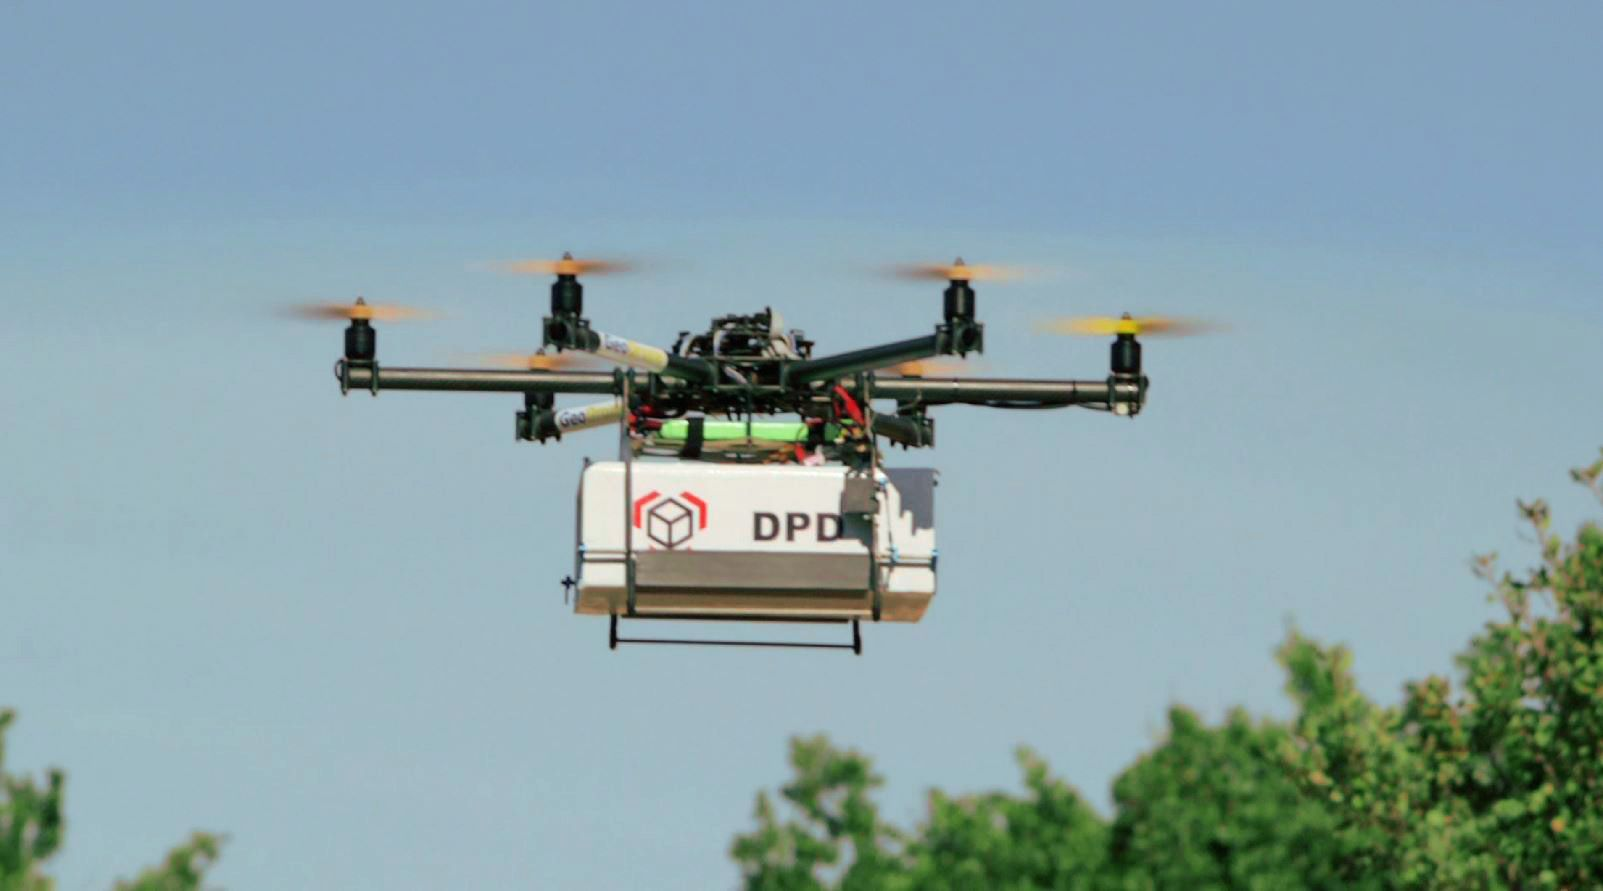
\includegraphics[width=5cm]{images/carrier-drone.jpg} }}%
    \qquad
    \subfloat[A fleet of drones such as on the left, coordinating to move a package from $S$ to $T$ in the least time possible.]{{\includegraphics[width=5cm]{example-image-b} }}%
    \caption{An instance of the Package Handoff problem for a single package}%
    \label{single-pho-example}%
\end{figure}


The challenge is to figure how to get the drones to cooperate to send 
the package from $S$ to $T$ in the least possible time i.e. minimize the makespan
of the delivery process. 

To solve the problem we need to be able to do several things

\begin{itemize}
\item Figure out which subset $S = \{i_1, i_2, \ldots i_k\}$ of the drones are used in the optimal schedule. 
\item Find the order in which the handoffs happend between the drones used in a schedule. 
\item Find the ``handoff'' points when drone $i_m$ hands over the package to drone $i_{m+1}$ for all $m \leq k-1$ 
      \footnote{The final drone $i_k$ in the schedule flies with the package to the target site $T$}
\end{itemize}

This category of problems is a generalization of computing shortest paths in $\mathbb{R}^2$ 
between 
two points. As far as we know such problems have not been considered before in the 
operations research or computational geometry literature; it is, however, reminescent of 
the Weighted Region Problem \cite{mitchell1991weighted} (henceforth abbreviated as 
\texttt{WRP}) where one needs to figure out how to compute a 
shortest \textit{weighted} path between two points in the plane
that has been partitioned into convex polygonal regions, each associated with a constant 
multiplicative weight for scaling the euclidean distance between two points 
\textit{within} that region.  


The distinctive feature of this problem and its generalizations is figuring out how 
to make multiple agents of \textit{varying} capabilities  located at different points 
in $\mathbb{R}^2$ (such as maximum capable speed, battery capacity, tethering constraints 
etc.) \textit{cooperate} in transporting one or more packages most efficiently 
from their given sources to their target destinations. 

While we are framing these problems in terms of drones, one can also apply this problem 
in routing a fleet of taxis to get passengers from their pickup to their dropoff locations. 
Interesting problems might arise in this scenario itself (e.g. what if the sequence of 
pickup and dropoff locations for passengers happen in an online manner, say when passengers request or cancel rides with their 
smartphones?) We leave the investigation of these latter fascinating problems for future work. 
All problems considered in this article are in the offline setting. 


Each chapter in this document is devoted to developing algorithms for a specific 
variant of the package handoff problem (henceforth abbreviated as \texttt{PHO}), beginning 
with the plain-vanilla single package handoff problem described above. 
For most algorithms we will also be giving implementations in Python described in a 
literate-programming style \footnote{Which essentially means you will see code-snippets interleaved with the actual explanation of the algorithms. 
The code snippets are then extracted using a literate programming tool (using a so-called a ``weaver'' and ``tangler'') into an 
executable Python program} \cite{knuth1984literate} using the NuWeb literate programming tool \cite{briggs2001nuweb}  
for weaving and tangling the code-snippets. 

You can check out the Package Handoff code from the following GitHub repository: 

\begin{center}
\url{https://github.com/gtelang/PackageHandoff_Python}
\end{center}

The \texttt{README} file in the repository gives instructions on how to run the code and any of the associated experiments. %-----------------------------------------------------
\chapter{Single Package Handoff}
\label{chap:single-package-handoff}

In this chapter, we consider the problem posed at the beginning of the Overview chapter. For convenience
we state the problem again below

\begin{displayquote}
Given the positions $P_i$ of $n$ drones (labelled 1 through $n$) 
in $\RR^2$ each capable of a maximum speed of $u_i \geq 0$. Also given is a package present 
at $S$ that needs to get to $T$. Each drone is capable of picking up the package and 
flying with speed $u_i$ to another point to hand the package off to another drone (which in turn 
hands the package off to another drone and so on). 
 
Find the best way to coordinate the movement of the drones to get the package from $S$ to $T$ in the least 
possible time i.e. minimize the makespan of the delivery process. 

\end{displayquote} 


Note that in the optimal schedule, it is easy to construct an example such that not all drones will necessarily participate
in getting the package from $S$ to $T$. The challenge is to figure out which subset of drones to use, 
along with the handoff points. 

However, the following observations are crucial for the development of algorithms in this chapter. 

\begin{flem}

\begin{enumerate}

   \item  For the single delivery package handoff problem,  a slower drone, 
          always hands off the package to a faster drone, in any optimal schedule. 
          Thus, once we \textit{know} which drones participate in the schedule, the order in which they participate in the handoff
          from start to finish is determined according to their speeds, sorted from lowest to highest. 
\footnote{This property is unfortunately 
not true when there are multiple packages to be delivered to their respective desitinations, even for the case where the sources
and targets for all the packages are the same. Examples where this happens are given in the next chapter.}
   
    \item All drones involved in the optimal schedule start moving at time $t=0$ at full speed along a straight line towards a handoff point . The drones not involved 
          can remain stationary since they don't participate in the package transport. 
    
    \item No drone waits on any other drone at the rendezvous points in any optimal schedule. i.e. if two drones rendezvous at some 
          point $H$, they arrive at $H$ are precisely the same time on the clock. 

    \item The path of the package is a monotonic piecewise straight polygonal curve with respect to the direction $\overrightharp{ST}$
          no matter what the intial positions $P_i$ or speeds $u_i$ of the drones. \footnote{We conjecture this property to be true 
          even for the case of multiple packages i.e. the path of travel of each package is monotonic with respect to the vectors $S_i T_i$'s}
\end{enumerate}


 \end{flem}


Before proceeding, we first fix some notation: 

\begin{itemize}
\item $(P_i, u_i)$ for $1 \leq i \leq n$ where $P_i \in \RR^2$ and $u_i \geq 0$, $S,T \in \RR^2$ respectively stand for the initial positions, speed, and source and target points for a package. 
\item $(S=H_{i_0}), H_{i_1} \ldots H_{i_k}$ for $0 \leq i_0, \ldots i_k \leq n$ stand for points where the drones with labels $i_0, \ldots i_k$ handle the package in that order. More precisely 
      $H_{i_j}$ is the point where drone $i_{j-1}$ hands off the package to drone $i_j$ for $1 \leq j \leq k$.  
\end{itemize}



\section{Wavefront Algorithms}
The algorithms in this section are inspired by the Continuous Dijkstra paradigm used in computing shortest paths for the Weighted Region Problem
and for computing euclidean shortest paths in the presence of polygonal obstacles \cite{mitchell1991weighted, mitchell1996shortest}. 
The approximation and locality properties of these heuristics are considered later in the chapter. 


The general idea is simple: consider expanding circular wavelets centered at the positions $P_i$, each expanding with speed $u_i$. The drones invovled in the schedule
are then calculated by observing how the wavelets interact in time. The various heuristics differ according to how the subset of drones involved in the delivery 
process is figured out based on nature of the ``wavefront'' used to keep track of the current tentative location of the package. 

Once this subset of drones is calculated,  we use convex optimization (via the convex optimization modelling language CVXPY \cite{diamond2016cvxpy}) 
to figure out \textit{exactly} the handoff points for the drones involved in transporting the package from the source to the destination. 

Precise details follow in the subsections below.


\subsection{Preliminary Data Structures} \hspace{10mm}

Before proceeding, lets design some housekeeping data-structures to 
represent the problem. The following data-structure simply maintains the 
information about the drones, the source and target used as input to the 
problem. To get a PHO tour for the package, algorithms are passed as 
first class values to the method \verb|get_tour| of this class. 

Note that each algorithm does its own plotting and animation in a separate matplotlib window 
if so requested via the boolean flags \verb|plot_tour_p| , and \verb|animate_tour_p|. If both 
animation and plotting are requested they are done in separate windows each. 

%{python-mode}%
\begin{flushleft} \small\label{scrap1}\raggedright\small
\NWtarget{nuweb6}{} $\langle\,${\itshape PHO Data Structures}\nobreak\ {\footnotesize {6}}$\,\rangle\equiv$
\vspace{-1ex}
\begin{list}{}{} \item
\mbox{}\verb@@\\
\mbox{}\verb@class Single_PHO_Input:@\\
\mbox{}\verb@    def __init__(self, drone_info = [] , source = None, target=None):@\\
\mbox{}\verb@           self.drone_info = drone_info @\\
\mbox{}\verb@           self.source     = source@\\
\mbox{}\verb@           self.target     = target@\\
\mbox{}\verb@@\\
\mbox{}\verb@    def get_drone_pis (self):@\\
\mbox{}\verb@           return [self.drone_info[idx][0] for idx in range(len(self.drone_info)) ]@\\
\mbox{}\verb@           @\\
\mbox{}\verb@    def get_drone_uis (self):@\\
\mbox{}\verb@           return [self.drone_info[idx][1] for idx in range(len(self.drone_info)) ]@\\
\mbox{}\verb@         @\\
\mbox{}\verb@    def get_tour(self, algo):@\\
\mbox{}\verb@           return algo( self.drone_info, self.source, self.target, @\\
\mbox{}\verb@                        plot_tour_p = True)@\\
\mbox{}\verb@@\\
\mbox{}\verb@    # Methods for \verb|ReverseHorseflyInput|@\\
\mbox{}\verb@    def clearAllStates (self):@\\
\mbox{}\verb@          self.drone_info = []@\\
\mbox{}\verb@          self.source = None@\\
\mbox{}\verb@          self.target = None@\\
\mbox{}\verb@@\\
\mbox{}\verb@@\\
\mbox{}\verb@@\\
\mbox{}\verb@@\\
\mbox{}\verb@@{\NWsep}
\end{list}
\vspace{-1.5ex}
\footnotesize
\begin{list}{}{\setlength{\itemsep}{-\parsep}\setlength{\itemindent}{-\leftmargin}}
\item \NWtxtMacroDefBy\ \NWlink{nuweb6}{6}\NWlink{nuweb7a}{, 7a}.
\item \NWtxtMacroRefIn\ \NWlink{nuweb15}{15}.
\item \NWtxtIdentsDefed\nobreak\  \verb@Single_PHO_Input@\nobreak\ \NWlink{nuweb10}{10}.
\item{}
\end{list}
\vspace{4ex}
\end{flushleft}
%{/python-mode}%

\subsection{One-Dimensional Greedy Wavefront} \hspace{10mm}

The followinf data-structure keeps track of a single wavelet expanding at uniform speed around a given center
starting at a particular clock time. 

%{python-mode}%
\begin{flushleft} \small
\begin{minipage}{\linewidth}\label{scrap2}\raggedright\small
\NWtarget{nuweb7a}{} $\langle\,${\itshape PHO Data Structures}\nobreak\ {\footnotesize {7a}}$\,\rangle\equiv$
\vspace{-1ex}
\begin{list}{}{} \item
\mbox{}\verb@@\\
\mbox{}\verb@class DroneWavelet:@\\
\mbox{}\verb@    def __init__(self, startposn, speed, drone_idx,  clock_time):@\\
\mbox{}\verb@          self.center          = startposn@\\
\mbox{}\verb@          self.speed           = speed@\\
\mbox{}\verb@          self.drone_label     = drone_idx@\\
\mbox{}\verb@          self.last_reset_time = clock_time@\\
\mbox{}\verb@@\\
\mbox{}\verb@    def get_center(self):@\\
\mbox{}\verb@          return self.center@\\
\mbox{}\verb@@\\
\mbox{}\verb@    def get_speed(self):@\\
\mbox{}\verb@          return self.speed@\\
\mbox{}\verb@@\\
\mbox{}\verb@    def get_associated_drone(self):@\\
\mbox{}\verb@          return self.drone_label@\\
\mbox{}\verb@@\\
\mbox{}\verb@    def wavelet_size(self, clock_time): # radius of the disk@\\
\mbox{}\verb@           return (clock_time - last_reset_time) * self.speed@\\
\mbox{}\verb@    @\\
\mbox{}\verb@    def reset_wavelet(self, center, clock_time):@\\
\mbox{}\verb@         self.center = center@\\
\mbox{}\verb@         self.last_reset_time = clock_time @\\
\mbox{}\verb@@\\
\mbox{}\verb@@{\NWsep}
\end{list}
\vspace{-1.5ex}
\footnotesize
\begin{list}{}{\setlength{\itemsep}{-\parsep}\setlength{\itemindent}{-\leftmargin}}
\item \NWtxtMacroDefBy\ \NWlink{nuweb6}{6}\NWlink{nuweb7a}{, 7a}.
\item \NWtxtMacroRefIn\ \NWlink{nuweb15}{15}.

\item{}
\end{list}
\end{minipage}\vspace{4ex}
\end{flushleft}
%{/python-mode}%


The following function simply calculates the time taken for a drone to move between two points at a given uniform speed. 

%{python-mode}%
\begin{flushleft} \small
\begin{minipage}{\linewidth}\label{scrap3}\raggedright\small
\NWtarget{nuweb7b}{} $\langle\,${\itshape PHO Algorithms}\nobreak\ {\footnotesize {7b}}$\,\rangle\equiv$
\vspace{-1ex}
\begin{list}{}{} \item
\mbox{}\verb@@\\
\mbox{}\verb@def time_of_travel(start, stop, speed):@\\
\mbox{}\verb@     start = np.asarray(start)@\\
\mbox{}\verb@     stop  = np.asarray(stop)@\\
\mbox{}\verb@    @\\
\mbox{}\verb@     return np.linalg.norm(stop-start)/speed@\\
\mbox{}\verb@@{\NWsep}
\end{list}
\vspace{-1.5ex}
\footnotesize
\begin{list}{}{\setlength{\itemsep}{-\parsep}\setlength{\itemindent}{-\leftmargin}}
\item \NWtxtMacroDefBy\ \NWlink{nuweb7b}{7b}\NWlink{nuweb7c}{c}\NWlink{nuweb9}{, 9}.
\item \NWtxtMacroRefIn\ \NWlink{nuweb15}{15}.

\item{}
\end{list}
\end{minipage}\vspace{4ex}
\end{flushleft}
%{/python-mode}%



%{python-mode}%
\begin{flushleft} \small\label{scrap4}\raggedright\small
\NWtarget{nuweb7c}{} $\langle\,${\itshape PHO Algorithms}\nobreak\ {\footnotesize {7c}}$\,\rangle\equiv$
\vspace{-1ex}
\begin{list}{}{} \item
\mbox{}\verb@@\\
\mbox{}\verb@def algo_odw(drone_info, source, target, @\\
\mbox{}\verb@             animate_tour_p = False,@\\
\mbox{}\verb@             plot_tour_p    = False):@\\
\mbox{}\verb@@\\
\mbox{}\verb@@\\
\mbox{}\verb@    from scipy.optimize import minimize@\\
\mbox{}\verb@@\\
\mbox{}\verb@    print Fore.CYAN, "\n==========================================================="@\\
\mbox{}\verb@    print            "Running the one dimensional wavefront algorithm (algo_odw) "@\\
\mbox{}\verb@    print            "===========================================================", Style.RESET_ALL@\\
\mbox{}\verb@@\\
\mbox{}\verb@    source = np.asarray(source)@\\
\mbox{}\verb@    target = np.asarray(target)@\\
\mbox{}\verb@    sthat  = (target-source)/np.linalg.norm(target-source) # unit vector pointing from source to target@\\
\mbox{}\verb@@\\
\mbox{}\verb@    # Intialize wavelets for all drones@\\
\mbox{}\verb@    numdrones  = len(drone_info)@\\
\mbox{}\verb@    clock_time = 0.0@\\
\mbox{}\verb@@\\
\mbox{}\verb@    drone_wavelets = []@\\
\mbox{}\verb@    for (initposn, speed), idx in zip(drone_info, range(numdrones)):@\\
\mbox{}\verb@         drone_wavelets.append(  DroneWavelet(initposn, speed, idx, clock_time)  )@\\
\mbox{}\verb@@\\
\mbox{}\verb@    # Find the drone which can get to the source the quickest@\\
\mbox{}\verb@    tmin = np.inf@\\
\mbox{}\verb@    imin = None@\\
\mbox{}\verb@    for idx in range(numdrones):@\\
\mbox{}\verb@         initdroneposn = drone_info[idx][0]@\\
\mbox{}\verb@         dronespeed    = drone_info[idx][1]@\\
\mbox{}\verb@         tmin_idx = time_of_travel(initdroneposn, source, dronespeed)@\\
\mbox{}\verb@    @\\
\mbox{}\verb@         if tmin_idx < tmin:@\\
\mbox{}\verb@             tmin = tmin_idx@\\
\mbox{}\verb@             imin = idx @\\
\mbox{}\verb@@\\
\mbox{}\verb@    # Reset wavelet for the drone which reached the source the fastest@\\
\mbox{}\verb@    clock_time = tmin@\\
\mbox{}\verb@    drone_wavelets[imin].reset_wavelet(source, clock_time)@\\
\mbox{}\verb@@\\
\mbox{}\verb@    current_package_handler_idx = imin@\\
\mbox{}\verb@    current_package_position = source@\\
\mbox{}\verb@@\\
\mbox{}\verb@    drone_pool = range(numdrones)@\\
\mbox{}\verb@    drone_pool.remove(imin) @\\
\mbox{}\verb@    used_drones = []@\\
\mbox{}\verb@@\\
\mbox{}\verb@    package_reached_p   = False@\\
\mbox{}\verb@    while not(package_reached_p):@\\
\mbox{}\verb@          time_to_target_without_help =\@\\
\mbox{}\verb@              np.linalg.norm((target-current_package_position))/drone_info[current_package_handler_idx][1]@\\
\mbox{}\verb@          tintercept_min     = np.inf@\\
\mbox{}\verb@          idx_intercept_min  = None@\\
\mbox{}\verb@@\\
\mbox{}\verb@          for idx in drone_pool:@\\
\mbox{}\verb@              # Calculate tintercept here via scipy@\\
\mbox{}\verb@              u1 = drone_info[current_package_handler_idx][1]@\\
\mbox{}\verb@              u2 = drone_info[idx][1]@\\
\mbox{}\verb@    @\\
\mbox{}\verb@              if u2 < u1:@\\
\mbox{}\verb@                  continue # there won't be any use of the slower drone u2 in speeding up the package delivery process. @\\
\mbox{}\verb@              else: @\\
\mbox{}\verb@                p1 = np.asarray(drone_info[idx][0])@\\
\mbox{}\verb@                p2 = np.asarray(drone_info[current_package_handler_idx][0]) @\\
\mbox{}\verb@           @\\
\mbox{}\verb@                d  = np.linalg.norm( p1 - p2 )@\\
\mbox{}\verb@    @\\
\mbox{}\verb@                veca  = target-p1@\\
\mbox{}\verb@                vecb  = p2 - p1  @\\
\mbox{}\verb@                costh = np.dot( veca, vecb ) / (np.linalg.norm(veca) * np.linalg.norm(vecb))@\\
\mbox{}\verb@@\\
\mbox{}\verb@                fun    = lambda t: t[0]@\\
\mbox{}\verb@                cons   = ({'type': 'ineq', 'fun': lambda t:  u2 + d - u1 * costh * (t[0]-clock_time)/t[0] },@\\
\mbox{}\verb@                          {'type': 'ineq', 'fun': lambda t:  u2 - d + u1 * costh * (t[0]-clock_time)/t[0] })@\\
\mbox{}\verb@    @\\
\mbox{}\verb@                res = minimize(fun, [clock_time] , method='SLSQP', bounds=[(clock_time, None)], constraints=cons ) @\\
\mbox{}\verb@@\\
\mbox{}\verb@                if res.success:@\\
\mbox{}\verb@                      print Fore.CYAN, "Yay! Solver converged in "      , res.nit@\\
\mbox{}\verb@@\\
\mbox{}\verb@                else :@\\
\mbox{}\verb@                      print Fore.RED, "Boo! Solver did not converge!", res.nit, " iterations."@\\
\mbox{}\verb@                      print res.status@\\
\mbox{}\verb@                      print res.message @\\
\mbox{}\verb@                @\\
\mbox{}\verb@                tintercept = res.x[0]@\\
\mbox{}\verb@@\\
\mbox{}\verb@                print res.x, tintercept, tintercept_min@\\
\mbox{}\verb@                print tintercept < tintercept_min@\\
\mbox{}\verb@                if tintercept < tintercept_min:@\\
\mbox{}\verb@                   tintercept_min    = tintercept@\\
\mbox{}\verb@                   idx_intercept_min = idx@\\
\mbox{}\verb@@\\
\mbox{}\verb@@\\
\mbox{}\verb@          if time_to_target_without_help < tintercept_min :@\\
\mbox{}\verb@              package_reached_p = True@\\
\mbox{}\verb@          else:@\\
\mbox{}\verb@@\\
\mbox{}\verb@              package_handler_speed     = drone_info[current_package_handler_idx][1] @\\
\mbox{}\verb@              current_package_position  = current_package_position + \@\\
\mbox{}\verb@                   package_handler_speed * (tintercept_min - clock_time) *  sthat@\\
\mbox{}\verb@@\\
\mbox{}\verb@              clock_time = tintercept_min @\\
\mbox{}\verb@@\\
\mbox{}\verb@              current_package_handler_idx = idx_intercept_min@\\
\mbox{}\verb@              drone_pool.remove(idx_intercept_min)@\\
\mbox{}\verb@              used_drones.append(idx_intercept_min)  @\\
\mbox{}\verb@@\\
\mbox{}\verb@              drone_wavelets[current_package_handler_idx].reset_wavelet(current_package_position, clock_time)@\\
\mbox{}\verb@@\\
\mbox{}\verb@    tour = algo_pho_exact_given_order_of_drones ( [drone_info[idx] for idx in used_drones],source,target )@\\
\mbox{}\verb@@\\
\mbox{}\verb@    if plot_tour_p:@\\
\mbox{}\verb@         print Fore.GREEN, "Plotting the computed tour", Style.RESET_ALL@\\
\mbox{}\verb@    @\\
\mbox{}\verb@    if animate_tour_p:@\\
\mbox{}\verb@         print Fore.CYAN, "Animating the computed tour", Style.RESET_ALL@\\
\mbox{}\verb@    @\\
\mbox{}\verb@    return tour@\\
\mbox{}\verb@@{\NWsep}
\end{list}
\vspace{-1.5ex}
\footnotesize
\begin{list}{}{\setlength{\itemsep}{-\parsep}\setlength{\itemindent}{-\leftmargin}}
\item \NWtxtMacroDefBy\ \NWlink{nuweb7b}{7b}\NWlink{nuweb7c}{c}\NWlink{nuweb9}{, 9}.
\item \NWtxtMacroRefIn\ \NWlink{nuweb15}{15}.
\item \NWtxtIdentsDefed\nobreak\  \verb@algo_odw@\nobreak\ \NWlink{nuweb10}{10}.\item \NWtxtIdentsUsed\nobreak\  \verb@algo_pho_exact_given_order_of_drones@\nobreak\ \NWlink{nuweb9}{9}.
\item{}
\end{list}
\vspace{4ex}
\end{flushleft}
%{/python-mode}%






%{python-mode}%
\begin{flushleft} \small
\begin{minipage}{\linewidth}\label{scrap5}\raggedright\small
\NWtarget{nuweb9}{} $\langle\,${\itshape PHO Algorithms}\nobreak\ {\footnotesize {9}}$\,\rangle\equiv$
\vspace{-1ex}
\begin{list}{}{} \item
\mbox{}\verb@@\\
\mbox{}\verb@def  algo_pho_exact_given_order_of_drones ( drone_info ,source, target ):@\\
\mbox{}\verb@    pass@\\
\mbox{}\verb@@\\
\mbox{}\verb@@{\NWsep}
\end{list}
\vspace{-1.5ex}
\footnotesize
\begin{list}{}{\setlength{\itemsep}{-\parsep}\setlength{\itemindent}{-\leftmargin}}
\item \NWtxtMacroDefBy\ \NWlink{nuweb7b}{7b}\NWlink{nuweb7c}{c}\NWlink{nuweb9}{, 9}.
\item \NWtxtMacroRefIn\ \NWlink{nuweb15}{15}.
\item \NWtxtIdentsDefed\nobreak\  \verb@algo_pho_exact_given_order_of_drones@\nobreak\ \NWlink{nuweb7c}{7c}.
\item{}
\end{list}
\end{minipage}\vspace{4ex}
\end{flushleft}
%{/python-mode}%




\newpage
\section{Run Handler associated with this Chapter}


%{python-mode}%
\begin{flushleft} \small\label{scrap6}\raggedright\small
\NWtarget{nuweb10}{} $\langle\,${\itshape PHO Run Handlers}\nobreak\ {\footnotesize {10}}$\,\rangle\equiv$
\vspace{-1ex}
\begin{list}{}{} \item
\mbox{}\verb@@\\
\mbox{}\verb@def single_pho_run_handler():@\\
\mbox{}\verb@ @\\
\mbox{}\verb@    def wrapperEnterRunPoints(fig, ax, run):@\\
\mbox{}\verb@      def _enterPoints(event):@\\
\mbox{}\verb@        @\\
\mbox{}\verb@        if event.name      == 'button_press_event'          and \@\\
\mbox{}\verb@           (event.button   == 1 or event.button == 3)       and \@\\
\mbox{}\verb@            event.dblclick == True and event.xdata  != None and event.ydata  != None:@\\
\mbox{}\verb@@\\
\mbox{}\verb@             if event.button == 1:  @\\
\mbox{}\verb@                 # Insert blue circle representing the initial position of a drone@\\
\mbox{}\verb@                 print Fore.GREEN@\\
\mbox{}\verb@                 newPoint = (event.xdata, event.ydata)@\\
\mbox{}\verb@                 speed    = float(raw_input('What speed do you want to set for the drone @{\tt @}\verb@ ' + str(newPoint)) + '\n')@\\
\mbox{}\verb@                 run.drone_info.append( (newPoint, speed) ) @\\
\mbox{}\verb@                 patchSize  = (xlim[1]-xlim[0])/40.0@\\
\mbox{}\verb@                 print Style.RESET_ALL@\\
\mbox{}\verb@                 @\\
\mbox{}\verb@                 ax.add_patch( mpl.patches.Circle( newPoint, radius = patchSize,@\\
\mbox{}\verb@                                                   facecolor='#b7e8cc', edgecolor='black'  ))@\\
\mbox{}\verb@@\\
\mbox{}\verb@                 ax.text( newPoint[0], newPoint[1], speed, fontsize=15, horizontalalignment='center', verticalalignment='center' )@\\
\mbox{}\verb@@\\
\mbox{}\verb@                 ax.set_title('Number of drones inserted: ' + str(len(run.drone_info)), fontdict={'fontsize':25})@\\
\mbox{}\verb@                 @\\
\mbox{}\verb@@\\
\mbox{}\verb@             elif event.button == 3:  @\\
\mbox{}\verb@                 # Insert big red circles representing the source and target points@\\
\mbox{}\verb@    @\\
\mbox{}\verb@                 patchSize  = (xlim[1]-xlim[0])/50.0@\\
\mbox{}\verb@                 if run.source is None:    @\\
\mbox{}\verb@                      run.source = (event.xdata, event.ydata)  @\\
\mbox{}\verb@                      ax.add_patch( mpl.patches.Circle( run.source, radius = patchSize, facecolor= '#ffd9d6', edgecolor='black', lw=1.0 ))@\\
\mbox{}\verb@                      ax.text( run.source[0], run.source[1], 'S', fontsize=15, horizontalalignment='center', verticalalignment='center' )@\\
\mbox{}\verb@@\\
\mbox{}\verb@                 elif run.target is None:@\\
\mbox{}\verb@                      run.target = (event.xdata, event.ydata)  @\\
\mbox{}\verb@                      ax.add_patch( mpl.patches.Circle( run.target, radius = patchSize, facecolor= '#ffd9d6', edgecolor='black', lw=1.0 ))@\\
\mbox{}\verb@                      ax.text( run.target[0], run.target[1], 'T', fontsize=15, horizontalalignment='center', verticalalignment='center' )@\\
\mbox{}\verb@    @\\
\mbox{}\verb@                 else:@\\
\mbox{}\verb@                       print Fore.RED, "Source and Target already set", Style.RESET_ALL@\\
\mbox{}\verb@@\\
\mbox{}\verb@@\\
\mbox{}\verb@             # Clear polygon patches and set up last minute \verb|ax| tweaks@\\
\mbox{}\verb@             clearAxPolygonPatches(ax)@\\
\mbox{}\verb@             applyAxCorrection(ax)@\\
\mbox{}\verb@             fig.canvas.draw()@\\
\mbox{}\verb@             @\\
\mbox{}\verb@@\\
\mbox{}\verb@      return _enterPoints@\\
\mbox{}\verb@@\\
\mbox{}\verb@    # The key-stack argument is mutable! I am using this hack to my advantage.@\\
\mbox{}\verb@    def wrapperkeyPressHandler(fig, ax, run): @\\
\mbox{}\verb@           def _keyPressHandler(event):@\\
\mbox{}\verb@               if event.key in ['i', 'I']:  @\\
\mbox{}\verb@@\\
\mbox{}\verb@                    # Select algorithm to execute@\\
\mbox{}\verb@                    algo_str = raw_input(Fore.YELLOW                                             +\@\\
\mbox{}\verb@                            "Enter algorithm to be used to compute the tour:\n Options are:\n"   +\@\\
\mbox{}\verb@                            " (odw)     One Dimensional Wavefront \n"                            +\@\\
\mbox{}\verb@                            Style.RESET_ALL)@\\
\mbox{}\verb@@\\
\mbox{}\verb@                    algo_str = algo_str.lstrip()@\\
\mbox{}\verb@                     @\\
\mbox{}\verb@                    # Incase there are patches present from the previous clustering, just clear them@\\
\mbox{}\verb@                    clearAxPolygonPatches(ax)@\\
\mbox{}\verb@@\\
\mbox{}\verb@                    if   algo_str == 'odw':@\\
\mbox{}\verb@                          tour = run.get_tour( algo_odw )@\\
\mbox{}\verb@                    else:@\\
\mbox{}\verb@                          print "Unknown option. No horsefly for you! ;-D "@\\
\mbox{}\verb@                          sys.exit()@\\
\mbox{}\verb@@\\
\mbox{}\verb@                    applyAxCorrection(ax)@\\
\mbox{}\verb@                    fig.canvas.draw()@\\
\mbox{}\verb@                    @\\
\mbox{}\verb@               elif event.key in ['c', 'C']: @\\
\mbox{}\verb@                    # Clear canvas and states of all objects@\\
\mbox{}\verb@                    run.clearAllStates()@\\
\mbox{}\verb@                    ax.cla()@\\
\mbox{}\verb@                                  @\\
\mbox{}\verb@                    utils_graphics.applyAxCorrection(ax)@\\
\mbox{}\verb@                    ax.set_xticks([])@\\
\mbox{}\verb@                    ax.set_yticks([])@\\
\mbox{}\verb@                                     @\\
\mbox{}\verb@                    fig.texts = []@\\
\mbox{}\verb@                    fig.canvas.draw()@\\
\mbox{}\verb@                    @\\
\mbox{}\verb@           return _keyPressHandler@\\
\mbox{}\verb@    @\\
\mbox{}\verb@    # Set up interactive canvas@\\
\mbox{}\verb@    fig, ax =  plt.subplots()@\\
\mbox{}\verb@    run = Single_PHO_Input()@\\
\mbox{}\verb@        @\\
\mbox{}\verb@    from matplotlib import rc@\\
\mbox{}\verb@    @\\
\mbox{}\verb@    # specify the custom font to use@\\
\mbox{}\verb@    plt.rcParams['font.family'] = 'sans-serif'@\\
\mbox{}\verb@    plt.rcParams['font.sans-serif'] = 'Times New Roman'@\\
\mbox{}\verb@@\\
\mbox{}\verb@    ax.set_xlim([xlim[0], xlim[1]])@\\
\mbox{}\verb@    ax.set_ylim([ylim[0], ylim[1]])@\\
\mbox{}\verb@    ax.set_aspect(1.0)@\\
\mbox{}\verb@    ax.set_xticks([])@\\
\mbox{}\verb@    ax.set_yticks([])@\\
\mbox{}\verb@          @\\
\mbox{}\verb@    ax.set_title("Enter drone positions, source and target onto canvas. \n (Enter speeds into the terminal, after inserting a drone at a particular position)")@\\
\mbox{}\verb@@\\
\mbox{}\verb@    mouseClick   = wrapperEnterRunPoints (fig,ax, run)@\\
\mbox{}\verb@    fig.canvas.mpl_connect('button_press_event' , mouseClick)@\\
\mbox{}\verb@          @\\
\mbox{}\verb@    keyPress     = wrapperkeyPressHandler(fig,ax, run)@\\
\mbox{}\verb@    fig.canvas.mpl_connect('key_press_event', keyPress   )@\\
\mbox{}\verb@    @\\
\mbox{}\verb@    plt.show()@\\
\mbox{}\verb@    @\\
\mbox{}\verb@@{\NWsep}
\end{list}
\vspace{-1.5ex}
\footnotesize
\begin{list}{}{\setlength{\itemsep}{-\parsep}\setlength{\itemindent}{-\leftmargin}}
\item \NWtxtMacroRefIn\ \NWlink{nuweb15}{15}.
\item \NWtxtIdentsDefed\nobreak\  \verb@single_pho_run_handler@\nobreak\ \NWlink{nuweb15}{15}.\item \NWtxtIdentsUsed\nobreak\  \verb@algo_odw@\nobreak\ \NWlink{nuweb7c}{7c}, \verb@Single_PHO_Input@\nobreak\ \NWlink{nuweb6}{6}.
\item{}
\end{list}
\vspace{4ex}
\end{flushleft}
%{/python-mode}%




\section{Chapter Index of Fragments}

{\small\begin{list}{}{\setlength{\itemsep}{-\parsep}\setlength{\itemindent}{-\leftmargin}}
\item $\langle\,$PHO Algorithms\nobreak\ {\footnotesize \NWlink{nuweb7b}{7b}\NWlink{nuweb7c}{c}\NWlink{nuweb9}{, 9}}$\,\rangle$ {\footnotesize {\NWtxtRefIn} \NWlink{nuweb15}{15}.}
\item $\langle\,$PHO Data Structures\nobreak\ {\footnotesize \NWlink{nuweb6}{6}\NWlink{nuweb7a}{, 7a}}$\,\rangle$ {\footnotesize {\NWtxtRefIn} \NWlink{nuweb15}{15}.}
\item $\langle\,$PHO Run Handlers\nobreak\ {\footnotesize \NWlink{nuweb10}{10}}$\,\rangle$ {\footnotesize {\NWtxtRefIn} \NWlink{nuweb15}{15}.}
\end{list}}
\section{Chapter Index of Identifiers}

{\small\begin{list}{}{\setlength{\itemsep}{-\parsep}\setlength{\itemindent}{-\leftmargin}}
\item \verb@algo_odw@: \underline{\NWlink{nuweb7c}{7c}}\NWlink{nuweb10}{, 10}.
\item \verb@algo_pho_exact_given_order_of_drones@: \NWlink{nuweb7c}{7c}, \underline{\NWlink{nuweb9}{9}}.
\item \verb@Single_PHO_Input@: \underline{\NWlink{nuweb6}{6}}\NWlink{nuweb10}{, 10}.
\item \verb@single_pho_run_handler@: \underline{\NWlink{nuweb10}{10}}\NWlink{nuweb15}{, 15}.
\end{list}} 
%------------------------------------------------------
\nocite{*} % include everything in the bibtex file
\bibliography{packagehandoff-main} 
\bibliographystyle{ieeetr}

\begin{appendices}
\chapter{Supporting Code}

\section{Main File}



%{python-mode}%
\begin{flushleft} \small\label{scrap7}\raggedright\small
\NWtarget{nuweb15}{} \verb@"../src/pho-main.py"@\nobreak\ {\footnotesize {15}}$\equiv$
\vspace{-1ex}
\begin{list}{}{} \item
\mbox{}\verb@@\\
\mbox{}\verb@# Relevant imports for Package Handoff@\\
\mbox{}\verb@@\\
\mbox{}\verb@from colorama import Fore, Style@\\
\mbox{}\verb@from matplotlib import rc@\\
\mbox{}\verb@from scipy.optimize import minimize@\\
\mbox{}\verb@from sklearn.cluster import KMeans@\\
\mbox{}\verb@import argparse@\\
\mbox{}\verb@import inspect @\\
\mbox{}\verb@import itertools@\\
\mbox{}\verb@import logging@\\
\mbox{}\verb@import math@\\
\mbox{}\verb@import matplotlib as mpl@\\
\mbox{}\verb@import matplotlib.pyplot as plt@\\
\mbox{}\verb@import numpy as np@\\
\mbox{}\verb@import os@\\
\mbox{}\verb@import pprint as pp@\\
\mbox{}\verb@import randomcolor @\\
\mbox{}\verb@import sys@\\
\mbox{}\verb@import time@\\
\mbox{}\verb@import utils_algo@\\
\mbox{}\verb@import utils_graphics@\\
\mbox{}\verb@@\\
\mbox{}\verb@@\hbox{$\langle\,${\itshape PHO Data Structures}\nobreak\ {\footnotesize \NWlink{nuweb6}{6}, \ldots\ }$\,\rangle$}\verb@@\\
\mbox{}\verb@@\hbox{$\langle\,${\itshape PHO Algorithms}\nobreak\ {\footnotesize \NWlink{nuweb7b}{7b}, \ldots\ }$\,\rangle$}\verb@@\\
\mbox{}\verb@@\hbox{$\langle\,${\itshape PHO Run Handlers}\nobreak\ {\footnotesize \NWlink{nuweb10}{10}}$\,\rangle$}\verb@@\\
\mbox{}\verb@@\\
\mbox{}\verb@# Set up logging information relevant to this module@\\
\mbox{}\verb@logger=logging.getLogger(__name__)@\\
\mbox{}\verb@logging.basicConfig(level=logging.DEBUG)@\\
\mbox{}\verb@@\\
\mbox{}\verb@def debug(msg):@\\
\mbox{}\verb@    frame,filename,line_number,function_name,lines,index=inspect.getouterframes(@\\
\mbox{}\verb@        inspect.currentframe())[1]@\\
\mbox{}\verb@    line=lines[0]@\\
\mbox{}\verb@    indentation_level=line.find(line.lstrip())@\\
\mbox{}\verb@    logger.debug('{i} [{m}]'.format(@\\
\mbox{}\verb@        i='.'*indentation_level, m=msg))@\\
\mbox{}\verb@@\\
\mbox{}\verb@@\\
\mbox{}\verb@def info(msg):@\\
\mbox{}\verb@    frame,filename,line_number,function_name,lines,index=inspect.getouterframes(@\\
\mbox{}\verb@        inspect.currentframe())[1]@\\
\mbox{}\verb@    line=lines[0]@\\
\mbox{}\verb@    indentation_level=line.find(line.lstrip())@\\
\mbox{}\verb@    logger.info('{i} [{m}]'.format(@\\
\mbox{}\verb@        i='.'*indentation_level, m=msg))@\\
\mbox{}\verb@@\\
\mbox{}\verb@xlim, ylim = [0,1], [0,1]@\\
\mbox{}\verb@@\\
\mbox{}\verb@def applyAxCorrection(ax):@\\
\mbox{}\verb@      ax.set_xlim([xlim[0], xlim[1]])@\\
\mbox{}\verb@      ax.set_ylim([ylim[0], ylim[1]])@\\
\mbox{}\verb@      ax.set_aspect(1.0)@\\
\mbox{}\verb@@\\
\mbox{}\verb@def clearPatches(ax):@\\
\mbox{}\verb@    # Get indices cooresponding to the polygon patches@\\
\mbox{}\verb@    for index , patch in zip(range(len(ax.patches)), ax.patches):@\\
\mbox{}\verb@        if isinstance(patch, mpl.patches.Polygon) == True:@\\
\mbox{}\verb@            patch.remove()@\\
\mbox{}\verb@    ax.lines[:]=[]@\\
\mbox{}\verb@    applyAxCorrection(ax)@\\
\mbox{}\verb@@\\
\mbox{}\verb@def clearAxPolygonPatches(ax):@\\
\mbox{}\verb@@\\
\mbox{}\verb@    # Get indices cooresponding to the polygon patches@\\
\mbox{}\verb@    for index , patch in zip(range(len(ax.patches)), ax.patches):@\\
\mbox{}\verb@        if isinstance(patch, mpl.patches.Polygon) == True:@\\
\mbox{}\verb@            patch.remove()@\\
\mbox{}\verb@    ax.lines[:]=[]@\\
\mbox{}\verb@    applyAxCorrection(ax)@\\
\mbox{}\verb@@\\
\mbox{}\verb@@\\
\mbox{}\verb@def animate_tour (sites, phi, horse_trajectories, fly_trajectories, @\\
\mbox{}\verb@                  animation_file_name_prefix, algo_name,  render_trajectory_trails_p = False):@\\
\mbox{}\verb@    """ This function can handle the animation of multiple@\\
\mbox{}\verb@    horses and flies even when the the fly trajectories are all squiggly@\\
\mbox{}\verb@    and if the flies have to wait at the end of their trajectories. @\\
\mbox{}\verb@    @\\
\mbox{}\verb@    A fly trajectory should only be a list of points! The sites are always the @\\
\mbox{}\verb@    first points on the trajectories. Any waiting for the flies, is assumed to be @\\
\mbox{}\verb@    at the end of their trajectories where it waits for the horse to come @\\
\mbox{}\verb@    and pick them up. @\\
\mbox{}\verb@@\\
\mbox{}\verb@    Every point on the horse trajectory stores a list of indices of the flies@\\
\mbox{}\verb@    collected at the end point. (The first point just stores the dummy value None). @\\
\mbox{}\verb@    Usually these index lists will be size 1, but there may be heuristics where you @\\
\mbox{}\verb@    might want to collect a bunch of them together since they may already be waiting @\\
\mbox{}\verb@    there at the pick up point. @\\
\mbox{}\verb@@\\
\mbox{}\verb@    For each drone collected, a yellow circle is placed on top of it, so that @\\
\mbox{}\verb@    it is marked as collected to be able to see the progress of the visualization @\\
\mbox{}\verb@    as it goes on. @\\
\mbox{}\verb@@\\
\mbox{}\verb@    """@\\
\mbox{}\verb@    import numpy as np@\\
\mbox{}\verb@    import matplotlib.animation as animation@\\
\mbox{}\verb@    from   matplotlib.patches import Circle@\\
\mbox{}\verb@    import matplotlib.pyplot as plt @\\
\mbox{}\verb@@\\
\mbox{}\verb@    # Set up configurations and parameters for all necessary graphics@\\
\mbox{}\verb@    plt.rc('text', usetex=True)@\\
\mbox{}\verb@    plt.rc('font', family='serif')@\\
\mbox{}\verb@@\\
\mbox{}\verb@    fig, ax = plt.subplots()@\\
\mbox{}\verb@    ax.set_xlim([0,1])@\\
\mbox{}\verb@    ax.set_ylim([0,1])@\\
\mbox{}\verb@    ax.set_aspect('equal')@\\
\mbox{}\verb@@\\
\mbox{}\verb@    ax.set_xticks(np.arange(0, 1, 0.1))@\\
\mbox{}\verb@    ax.set_yticks(np.arange(0, 1, 0.1))@\\
\mbox{}\verb@@\\
\mbox{}\verb@    # Turn on the minor TICKS, which are required for the minor GRID@\\
\mbox{}\verb@    ax.minorticks_on()@\\
\mbox{}\verb@@\\
\mbox{}\verb@    # customize the major grid@\\
\mbox{}\verb@    ax.grid(which='major', linestyle='--', linewidth='0.3', color='red')@\\
\mbox{}\verb@@\\
\mbox{}\verb@    # Customize the minor grid@\\
\mbox{}\verb@    ax.grid(which='minor', linestyle=':', linewidth='0.3', color='black')@\\
\mbox{}\verb@@\\
\mbox{}\verb@    ax.get_xaxis().set_ticklabels([])@\\
\mbox{}\verb@    ax.get_yaxis().set_ticklabels([])@\\
\mbox{}\verb@@\\
\mbox{}\verb@    mspan, _ = makespan(horse_trajectories)@\\
\mbox{}\verb@    ax.set_title("Algo: " + algo_name + "  Makespan: " + '%.4f' % mspan , fontsize=25)@\\
\mbox{}\verb@@\\
\mbox{}\verb@    number_of_flies  = len(fly_trajectories)@\\
\mbox{}\verb@    number_of_horses = len(horse_trajectories)@\\
\mbox{}\verb@    colors           = utils_graphics.get_colors(number_of_horses, lightness=0.5)@\\
\mbox{}\verb@        @\\
\mbox{}\verb@    ax.set_xlabel( "Number of drones: " + str(number_of_flies) + "\n" + r"$\varphi=$ " + str(phi), fontsize=25)@\\
\mbox{}\verb@    ims                = []@\\
\mbox{}\verb@    @\\
\mbox{}\verb@    # Constant for discretizing each segment inside the trajectories of the horses@\\
\mbox{}\verb@    # and flies. @\\
\mbox{}\verb@    NUM_SUB_LEGS              = 2 # Number of subsegments within each segment of every trajectory@\\
\mbox{}\verb@    @\\
\mbox{}\verb@    # Arrays keeping track of the states of the horses@\\
\mbox{}\verb@    horses_reached_endpt_p    = [False for i in range(number_of_horses)]@\\
\mbox{}\verb@    horses_traj_num_legs      = [len(traj)-1 for traj in horse_trajectories] # the -1 is because the initial position of the horse is always included. @\\
\mbox{}\verb@    horses_current_leg_idx    = [0 for i in range(number_of_horses)]@\\
\mbox{}\verb@    horses_current_subleg_idx = [0 for i in range(number_of_horses)] @\\
\mbox{}\verb@    horses_current_posn       = [traj[0]['coords'] for traj in horse_trajectories]@\\
\mbox{}\verb@@\\
\mbox{}\verb@    # List of arrays keeping track of the flies collected by the horses at any given point in time, @\\
\mbox{}\verb@    fly_idxs_collected_so_far = [[] for i in range(number_of_horses)] @\\
\mbox{}\verb@@\\
\mbox{}\verb@    # Arrays keeping track of the states of the flies@\\
\mbox{}\verb@    flies_reached_endpt_p    = [False for i in range(number_of_flies)]@\\
\mbox{}\verb@    flies_traj_num_legs      = [len(traj)-1 for traj in fly_trajectories]@\\
\mbox{}\verb@    flies_current_leg_idx    = [0 for i in range(number_of_flies)]@\\
\mbox{}\verb@    flies_current_subleg_idx = [0 for i in range(number_of_flies)] @\\
\mbox{}\verb@    flies_current_posn       = [traj[0] for traj in fly_trajectories]@\\
\mbox{}\verb@@\\
\mbox{}\verb@    # The drone collection process ends, when all the flies AND horses @\\
\mbox{}\verb@    # have reached their ends. Some heuristics, might involve the flies @\\
\mbox{}\verb@    # or the horses waiting at the endpoints of their respective trajectories. @\\
\mbox{}\verb@    image_frame_counter = 0@\\
\mbox{}\verb@    while not(all(horses_reached_endpt_p + flies_reached_endpt_p)): @\\
\mbox{}\verb@@\\
\mbox{}\verb@        # Update the states of all the horses@\\
\mbox{}\verb@        for hidx in range(number_of_horses):@\\
\mbox{}\verb@            if horses_reached_endpt_p[hidx] == False:@\\
\mbox{}\verb@                htraj                       = [elt['coords'] for elt in horse_trajectories[hidx]]@\\
\mbox{}\verb@                all_flys_collected_by_horse = [i             for elt in horse_trajectories[hidx] for i in elt['fly_idxs_picked_up']]@\\
\mbox{}\verb@@\\
\mbox{}\verb@                if horses_current_subleg_idx[hidx] <= NUM_SUB_LEGS-2:@\\
\mbox{}\verb@@\\
\mbox{}\verb@                    horses_current_subleg_idx[hidx] += 1     # subleg idx changes@\\
\mbox{}\verb@                    legidx    = horses_current_leg_idx[hidx] # the legidx remains the same@\\
\mbox{}\verb@                    @\\
\mbox{}\verb@                    sublegidx = horses_current_subleg_idx[hidx] # shorthand for easier reference in the next two lines@\\
\mbox{}\verb@                    xcurr = np.linspace( htraj[legidx][0], htraj[legidx+1][0], NUM_SUB_LEGS+1 )[sublegidx]@\\
\mbox{}\verb@                    ycurr = np.linspace( htraj[legidx][1], htraj[legidx+1][1], NUM_SUB_LEGS+1 )[sublegidx]@\\
\mbox{}\verb@                    horses_current_posn[hidx]  = [xcurr, ycurr] @\\
\mbox{}\verb@@\\
\mbox{}\verb@                    @\\
\mbox{}\verb@                else:@\\
\mbox{}\verb@                    horses_current_subleg_idx[hidx] = 0 # reset to 0@\\
\mbox{}\verb@                    horses_current_leg_idx[hidx]   += 1 # you have passed onto the next leg@\\
\mbox{}\verb@                    legidx    = horses_current_leg_idx[hidx]@\\
\mbox{}\verb@@\\
\mbox{}\verb@                    xcurr, ycurr = htraj[legidx][0], htraj[legidx][1] # current position is the zeroth point on the next leg@\\
\mbox{}\verb@                    horses_current_posn[hidx]  = [xcurr , ycurr] @\\
\mbox{}\verb@@\\
\mbox{}\verb@                    if horses_current_leg_idx[hidx] == horses_traj_num_legs[hidx]:@\\
\mbox{}\verb@                        horses_reached_endpt_p[hidx] = True@\\
\mbox{}\verb@@\\
\mbox{}\verb@                ####################......for marking in yellow during rendering@\\
\mbox{}\verb@                fly_idxs_collected_so_far[hidx].extend(horse_trajectories[hidx][legidx]['fly_idxs_picked_up'])@\\
\mbox{}\verb@                fly_idxs_collected_so_far[hidx] = list(set(fly_idxs_collected_so_far[hidx])) ### critical line, to remove duplicate elements # https://stackoverflow.com/a/7961390@\\
\mbox{}\verb@@\\
\mbox{}\verb@        # Update the states of all the flies@\\
\mbox{}\verb@        for fidx in range(number_of_flies):@\\
\mbox{}\verb@            if flies_reached_endpt_p[fidx] == False:@\\
\mbox{}\verb@                ftraj  = fly_trajectories[fidx]@\\
\mbox{}\verb@@\\
\mbox{}\verb@                if flies_current_subleg_idx[fidx] <= NUM_SUB_LEGS-2:@\\
\mbox{}\verb@                    @\\
\mbox{}\verb@                    flies_current_subleg_idx[fidx] += 1@\\
\mbox{}\verb@                    legidx    = flies_current_leg_idx[fidx]@\\
\mbox{}\verb@@\\
\mbox{}\verb@                    sublegidx = flies_current_subleg_idx[fidx]@\\
\mbox{}\verb@                    xcurr = np.linspace( ftraj[legidx][0], ftraj[legidx+1][0], NUM_SUB_LEGS+1 )[sublegidx]@\\
\mbox{}\verb@                    ycurr = np.linspace( ftraj[legidx][1], ftraj[legidx+1][1], NUM_SUB_LEGS+1 )[sublegidx]@\\
\mbox{}\verb@                    flies_current_posn[fidx]  = [xcurr, ycurr] @\\
\mbox{}\verb@@\\
\mbox{}\verb@                else:@\\
\mbox{}\verb@                    flies_current_subleg_idx[fidx] = 0 # reset to zero@\\
\mbox{}\verb@                    flies_current_leg_idx[fidx]   += 1 # you have passed onto the next leg@\\
\mbox{}\verb@                    legidx    = flies_current_leg_idx[fidx]@\\
\mbox{}\verb@@\\
\mbox{}\verb@                    xcurr, ycurr = ftraj[legidx][0], ftraj[legidx][1] # current position is the zeroth point on the next leg@\\
\mbox{}\verb@                    flies_current_posn[fidx]  = [xcurr , ycurr] @\\
\mbox{}\verb@@\\
\mbox{}\verb@                    if flies_current_leg_idx[fidx] == flies_traj_num_legs[fidx]:@\\
\mbox{}\verb@                        flies_reached_endpt_p[fidx] = True@\\
\mbox{}\verb@@\\
\mbox{}\verb@        objs = []@\\
\mbox{}\verb@        # Render all the horse trajectories uptil this point in time. @\\
\mbox{}\verb@        for hidx in range(number_of_horses):@\\
\mbox{}\verb@            traj               = [elt['coords'] for elt in horse_trajectories[hidx]]@\\
\mbox{}\verb@            current_horse_posn = horses_current_posn[hidx]@\\
\mbox{}\verb@            @\\
\mbox{}\verb@            if horses_current_leg_idx[hidx] != horses_traj_num_legs[hidx]: # the horse is still moving@\\
\mbox{}\verb@@\\
\mbox{}\verb@                  xhs = [traj[k][0] for k in range(1+horses_current_leg_idx[hidx])] + [current_horse_posn[0]]@\\
\mbox{}\verb@                  yhs = [traj[k][1] for k in range(1+horses_current_leg_idx[hidx])] + [current_horse_posn[1]]@\\
\mbox{}\verb@@\\
\mbox{}\verb@            else: # The horse has stopped moving@\\
\mbox{}\verb@                  xhs = [x for (x,y) in traj]@\\
\mbox{}\verb@                  yhs = [y for (x,y) in traj]@\\
\mbox{}\verb@@\\
\mbox{}\verb@            horseline, = ax.plot(xhs,yhs,'-',linewidth=5.0, markersize=6, alpha=0.80, color='#D13131')@\\
\mbox{}\verb@            horseloc   = Circle((current_horse_posn[0], current_horse_posn[1]), 0.015, facecolor = '#D13131', edgecolor='k',  alpha=1.00)@\\
\mbox{}\verb@            horsepatch = ax.add_patch(horseloc)@\\
\mbox{}\verb@            objs.append(horseline)@\\
\mbox{}\verb@            objs.append(horsepatch)@\\
\mbox{}\verb@@\\
\mbox{}\verb@        # Render all fly trajectories uptil this point in time@\\
\mbox{}\verb@        for fidx in range(number_of_flies):@\\
\mbox{}\verb@            traj               = fly_trajectories[fidx]@\\
\mbox{}\verb@            current_fly_posn   = flies_current_posn[fidx]@\\
\mbox{}\verb@            @\\
\mbox{}\verb@            if flies_current_leg_idx[fidx] != flies_traj_num_legs[fidx]: # the fly is still moving@\\
\mbox{}\verb@@\\
\mbox{}\verb@                  xfs = [traj[k][0] for k in range(1+flies_current_leg_idx[fidx])] + [current_fly_posn[0]]@\\
\mbox{}\verb@                  yfs = [traj[k][1] for k in range(1+flies_current_leg_idx[fidx])] + [current_fly_posn[1]]@\\
\mbox{}\verb@@\\
\mbox{}\verb@            else: # The fly has stopped moving@\\
\mbox{}\verb@                  xfs = [x for (x,y) in traj]@\\
\mbox{}\verb@                  yfs = [y for (x,y) in traj]@\\
\mbox{}\verb@@\\
\mbox{}\verb@            if render_trajectory_trails_p:@\\
\mbox{}\verb@                flyline, = ax.plot(xfs,yfs,'-',linewidth=2.5, markersize=6, alpha=0.32, color='b')@\\
\mbox{}\verb@                objs.append(flyline)@\\
\mbox{}\verb@@\\
\mbox{}\verb@@\\
\mbox{}\verb@            # If the current fly is in the list of flies already collected by some horse, @\\
\mbox{}\verb@            # mark this fly with yellow. If it hasn't been serviced yet, mark it with blue@\\
\mbox{}\verb@            service_status_col = 'b'@\\
\mbox{}\verb@            for hidx in range(number_of_horses):@\\
\mbox{}\verb@                #print fly_idxs_collected_so_far[hidx]@\\
\mbox{}\verb@                if fidx in fly_idxs_collected_so_far[hidx]:@\\
\mbox{}\verb@                    service_status_col = 'y'@\\
\mbox{}\verb@                    break@\\
\mbox{}\verb@@\\
\mbox{}\verb@            flyloc   = Circle((current_fly_posn[0], current_fly_posn[1]), 0.013, @\\
\mbox{}\verb@                              facecolor = service_status_col, edgecolor='k', alpha=1.00)@\\
\mbox{}\verb@            flypatch = ax.add_patch(flyloc)@\\
\mbox{}\verb@            objs.append(flypatch)@\\
\mbox{}\verb@        @\\
\mbox{}\verb@        print "........................"@\\
\mbox{}\verb@        print "Appending to ims ", image_frame_counter@\\
\mbox{}\verb@        ims.append(objs) @\\
\mbox{}\verb@        image_frame_counter += 1@\\
\mbox{}\verb@@\\
\mbox{}\verb@    from colorama import Back @\\
\mbox{}\verb@   @\\
\mbox{}\verb@    debug(Fore.BLACK + Back.WHITE + "\nStarted constructing ani object"+ Style.RESET_ALL)@\\
\mbox{}\verb@    ani = animation.ArtistAnimation(fig, ims, interval=70, blit=True, repeat=True, repeat_delay=500)@\\
\mbox{}\verb@    debug(Fore.BLACK + Back.WHITE + "\nFinished constructing ani object"+ Style.RESET_ALL)@\\
\mbox{}\verb@@\\
\mbox{}\verb@    debug(Fore.MAGENTA + "\nStarted writing animation to disk"+ Style.RESET_ALL)@\\
\mbox{}\verb@    #ani.save(animation_file_name_prefix+'.avi', dpi=100)@\\
\mbox{}\verb@    #ani.save('reverse_horsefly.avi', dpi=300)@\\
\mbox{}\verb@    debug(Fore.MAGENTA + "\nFinished writing animation to disk"+ Style.RESET_ALL)@\\
\mbox{}\verb@@\\
\mbox{}\verb@    plt.show()@\\
\mbox{}\verb@@\\
\mbox{}\verb@if __name__=="__main__":@\\
\mbox{}\verb@     print "Running Package Handoff"@\\
\mbox{}\verb@     single_pho_run_handler()@\\
\mbox{}\verb@@\\
\mbox{}\verb@@{\NWsep}
\end{list}
\vspace{-1.5ex}
\footnotesize
\begin{list}{}{\setlength{\itemsep}{-\parsep}\setlength{\itemindent}{-\leftmargin}}
\item \NWtxtIdentsUsed\nobreak\  \verb@single_pho_run_handler@\nobreak\ \NWlink{nuweb10}{10}.
\item{}
\end{list}
\vspace{4ex}
\end{flushleft}
%{/python-mode}%


\section{Algorithmic Utilities}

%{python-mode}%
\begin{flushleft} \small\label{scrap8}\raggedright\small
\NWtarget{nuweb20}{} \verb@"../src/utils_algo.py"@\nobreak\ {\footnotesize {20}}$\equiv$
\vspace{-1ex}
\begin{list}{}{} \item
\mbox{}\verb@    @\\
\mbox{}\verb@ @\\
\mbox{}\verb@import numpy as np@\\
\mbox{}\verb@import random@\\
\mbox{}\verb@from colorama import Fore@\\
\mbox{}\verb@from colorama import Style@\\
\mbox{}\verb@@\\
\mbox{}\verb@def vector_chain_from_point_list(pts):@\\
\mbox{}\verb@    vec_chain = []@\\
\mbox{}\verb@    for pair in zip(pts, pts[1:]):@\\
\mbox{}\verb@        tail= np.array (pair[0])@\\
\mbox{}\verb@        head= np.array (pair[1])@\\
\mbox{}\verb@        vec_chain.append(head-tail)@\\
\mbox{}\verb@@\\
\mbox{}\verb@    return vec_chain@\\
\mbox{}\verb@@\\
\mbox{}\verb@def length_polygonal_chain(pts):@\\
\mbox{}\verb@    vec_chain = vector_chain_from_point_list(pts)@\\
\mbox{}\verb@@\\
\mbox{}\verb@    acc = 0@\\
\mbox{}\verb@    for vec in vec_chain:@\\
\mbox{}\verb@        acc = acc + np.linalg.norm(vec)@\\
\mbox{}\verb@    return acc@\\
\mbox{}\verb@def pointify_vector (x):@\\
\mbox{}\verb@    if len(x) % 2 == 0:@\\
\mbox{}\verb@        pts = []@\\
\mbox{}\verb@        for i in range(len(x))[::2]:@\\
\mbox{}\verb@            pts.append( [x[i],x[i+1]] )@\\
\mbox{}\verb@        return pts@\\
\mbox{}\verb@    else :@\\
\mbox{}\verb@        sys.exit('List of items does not have an even length to be able to be pointifyed')@\\
\mbox{}\verb@def flatten_list_of_lists(l):@\\
\mbox{}\verb@       return [item for sublist in l for item in sublist]@\\
\mbox{}\verb@def print_list(xs):@\\
\mbox{}\verb@    for x in xs:@\\
\mbox{}\verb@        print x@\\
\mbox{}\verb@def partial_sums( xs ):@\\
\mbox{}\verb@    psum = 0@\\
\mbox{}\verb@    acc = []@\\
\mbox{}\verb@    for x in xs:@\\
\mbox{}\verb@        psum = psum+x@\\
\mbox{}\verb@        acc.append( psum )@\\
\mbox{}\verb@    return acc@\\
\mbox{}\verb@def are_site_orderings_equal(sites1, sites2):@\\
\mbox{}\verb@@\\
\mbox{}\verb@    for (x1,y1), (x2,y2) in zip(sites1, sites2): @\\
\mbox{}\verb@        if (x1-x2)**2 + (y1-y2)**2 > 1e-8:@\\
\mbox{}\verb@            return False@\\
\mbox{}\verb@    return True@\\
\mbox{}\verb@def bunch_of_non_uniform_random_points(numpts):@\\
\mbox{}\verb@    cluster_size = int(np.sqrt(numpts)) @\\
\mbox{}\verb@    numcenters   = cluster_size@\\
\mbox{}\verb@    @\\
\mbox{}\verb@    import scipy@\\
\mbox{}\verb@    import random@\\
\mbox{}\verb@    centers = scipy.rand(numcenters,2).tolist()@\\
\mbox{}\verb@@\\
\mbox{}\verb@    scale, points = 4.0, []@\\
\mbox{}\verb@    for c in centers:@\\
\mbox{}\verb@        cx, cy = c[0], c[1]@\\
\mbox{}\verb@        # For current center $c$ of this loop, generate \verb|cluster_size| points uniformly in a square centered at it@\\
\mbox{}\verb@           @\\
\mbox{}\verb@        sq_size      = min(cx,1-cx,cy, 1-cy)@\\
\mbox{}\verb@        loc_pts_x    = np.random.uniform(low=cx-sq_size/scale, high=cx+sq_size/scale, size=(cluster_size,))@\\
\mbox{}\verb@        loc_pts_y    = np.random.uniform(low=cy-sq_size/scale, high=cy+sq_size/scale, size=(cluster_size,))@\\
\mbox{}\verb@        points.extend(zip(loc_pts_x, loc_pts_y))@\\
\mbox{}\verb@        @\\
\mbox{}\verb@@\\
\mbox{}\verb@    # Whatever number of points are left to be generated, generate them uniformly inside the unit-square@\\
\mbox{}\verb@       @\\
\mbox{}\verb@    num_remaining_pts = numpts - cluster_size * numcenters@\\
\mbox{}\verb@    remaining_pts = scipy.rand(num_remaining_pts, 2).tolist()@\\
\mbox{}\verb@    points.extend(remaining_pts)@\\
\mbox{}\verb@    @\\
\mbox{}\verb@@\\
\mbox{}\verb@    return points@\\
\mbox{}\verb@    @\\
\mbox{}\verb@def write_to_yaml_file(data, dir_name, file_name):@\\
\mbox{}\verb@   import yaml@\\
\mbox{}\verb@   with open(dir_name + '/' + file_name, 'w') as outfile:@\\
\mbox{}\verb@     yaml.dump( data, outfile, default_flow_style = False)@\\
\mbox{}\verb@ @\\
\mbox{}\verb@@\\
\mbox{}\verb@@{\NWsep}
\end{list}
\vspace{-1.5ex}
\footnotesize
\begin{list}{}{\setlength{\itemsep}{-\parsep}\setlength{\itemindent}{-\leftmargin}}

\item{}
\end{list}
\vspace{4ex}
\end{flushleft}
%{/python-mode}%



\section{Graphical Utilities}


%{python-mode}%
\begin{flushleft} \small\label{scrap9}\raggedright\small
\NWtarget{nuweb21}{} \verb@"../src/utils_graphics.py"@\nobreak\ {\footnotesize {21}}$\equiv$
\vspace{-1ex}
\begin{list}{}{} \item
\mbox{}\verb@    @\\
\mbox{}\verb@@\\
\mbox{}\verb@from matplotlib import rc@\\
\mbox{}\verb@from colorama import Fore@\\
\mbox{}\verb@from colorama import Style@\\
\mbox{}\verb@from scipy.optimize import minimize@\\
\mbox{}\verb@from sklearn.cluster import KMeans@\\
\mbox{}\verb@import argparse@\\
\mbox{}\verb@import itertools@\\
\mbox{}\verb@import math@\\
\mbox{}\verb@import matplotlib as mpl@\\
\mbox{}\verb@import matplotlib.pyplot as plt@\\
\mbox{}\verb@import numpy as np@\\
\mbox{}\verb@import os@\\
\mbox{}\verb@import pprint as pp@\\
\mbox{}\verb@import randomcolor @\\
\mbox{}\verb@import sys@\\
\mbox{}\verb@import time@\\
\mbox{}\verb@@\\
\mbox{}\verb@xlim, ylim = [0,1], [0,1]@\\
\mbox{}\verb@@\\
\mbox{}\verb@# Borrowed from https://stackoverflow.com/a/9701141@\\
\mbox{}\verb@import numpy as np@\\
\mbox{}\verb@import colorsys@\\
\mbox{}\verb@@\\
\mbox{}\verb@def get_colors(num_colors, lightness=0.2):@\\
\mbox{}\verb@    colors=[]@\\
\mbox{}\verb@    for i in np.arange(60., 360., 300. / num_colors):@\\
\mbox{}\verb@        hue        = i/360.0@\\
\mbox{}\verb@        saturation = 0.95@\\
\mbox{}\verb@        colors.append(colorsys.hls_to_rgb(hue, lightness, saturation))@\\
\mbox{}\verb@    return colors@\\
\mbox{}\verb@@{\NWsep}
\end{list}
\vspace{-1.5ex}
\footnotesize
\begin{list}{}{\setlength{\itemsep}{-\parsep}\setlength{\itemindent}{-\leftmargin}}

\item{}
\end{list}
\vspace{4ex}
\end{flushleft}
%{/python-mode}%
\end{appendices}

\end{document}
